
\chapter{Analyse der Arbeit auf der Basis der Aufgabenstellung}\label{analyse}
\section{Zielerreichung Prototyp}
\subsection{Funktionsumfang f\"ur anonyme Benutzer}

Auf den folgenden drei Bildern sind die \"offentlichen Seiten des Prototypen abgebildet. Es handelt sich also um Funktionen die allen Benutzern zur Verf\"ugung stehen, sofern sie nicht angemeldet sind. Die Funktionalit\"aten sind grunds\"atzlich fertig implementiert, br\"auchten aber f\"ur eine produktive Anwendung noch einige Anpassungen:
\begin{itemize}
\item Mit dem Gedanken im Hinterkopf, dass es sich um einen Prototypen handelt, habe ich den Fokus weg vom grafischen Design genommen und mich auf den Funktionsumfang konzentriert. Hier w\"are es f\"ur eine produktive Applikation wichtig, noch einige Zeit zu investieren.
\item Der Code der Klasse BasicUser m\"usste \"uberarbeitet werden.
\item F\"ur eine mehrsprachige Anwendung m\"usste man die bestehenden Texte extrahieren und durch mehrsprachige Properties-Dateien ersetzen.
\end{itemize}

\begin{figure}[H]
  	\centering
    	\fbox{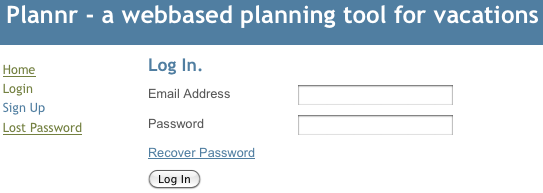
\includegraphics[width=10cm]{images/login}}
        	\caption{Login}
\end{figure}

\begin{figure}[H]
  	\centering
    	\fbox{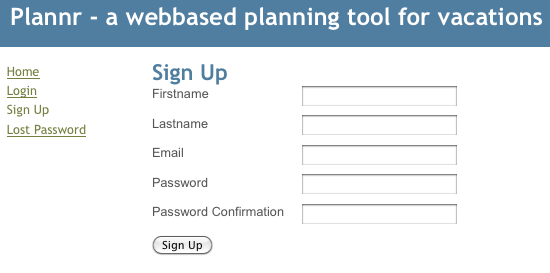
\includegraphics[width=10cm]{images/signup}}
        	\caption{Registrierung}
\end{figure}

 \begin{figure}[H]
  	\centering
    	\fbox{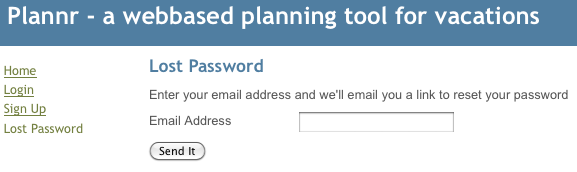
\includegraphics[width=10cm]{images/lost_password}}
        	\caption{Lost Password}
\end{figure}

\subsection{Funktionsumfang f\"ur registrierte Benutzer}
Nun kommen wir zu den Seiten, die nur dem angemeldeten Benutzer zur Verf\"ugung stehen. Die Seiten zur Benutzeradministration und \"Anderung des Passworts sind ebenfalls in HTML und CSS umgesetzt.

 \begin{figure}[H]
  	\centering
    	\fbox{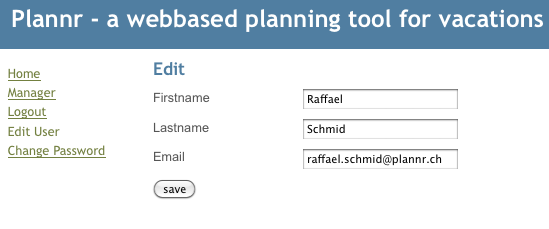
\includegraphics[width=10cm]{images/edit_user}}
        	\caption{Edit User}
\end{figure}

 \begin{figure}[H]
  	\centering
    	\fbox{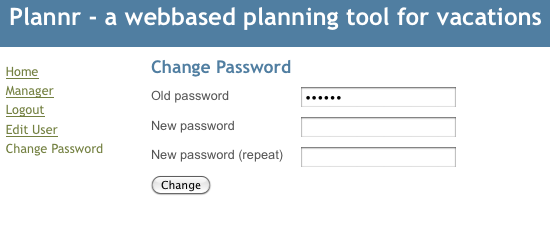
\includegraphics[width=10cm]{images/change_password}}
        	\caption{Change Password}
\end{figure}

Ab hier sind die Funktionalit\"aten der in Flex implementierten Seiten Teamadministration und Kalender abgebildet. Im Grossen und Ganzen sind die Anforderungen funktional implementiert. \textbf{Hingegen funktioniert die Freischaltung durch den Administrator noch nicht - Ferien k\"onnen zwar erfasst, editiert und gel\"oscht werden, hingegen k\"onnen die Ferien seitens Administrator noch nicht freigeschaltet werden. Es ist mir ein Dorn im Auge, aber ich musste die daf\"ur notwendige Zeit in die Dokumentation und die Umstellung der Architektur auf Dependency Injection investieren und kam nicht mehr zur Fertigstellung dieses Use Cases. }

 \begin{figure}[H]
  	\centering
    	\fbox{
\includegraphics[width=15cm]{images/calendar}}
        	\caption{Ferienplanung}
\end{figure}

 \begin{figure}[H]
  	\centering
    	\fbox{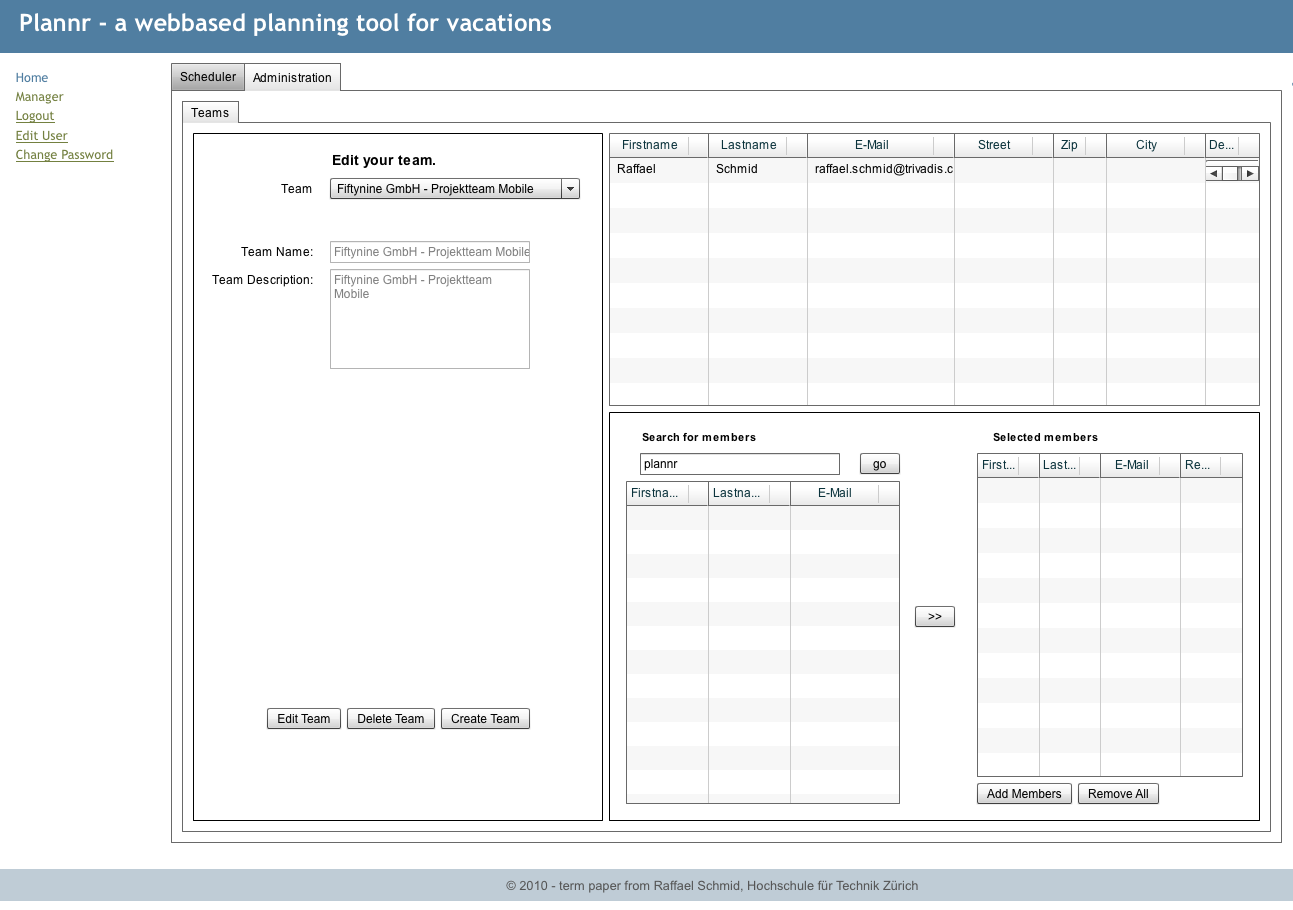
\includegraphics[width=15cm]{images/teams}}
        	\caption{Teamadministration}
\end{figure}

\section{Optionale Ziele Prototyp}
Die von mir in der Aufgabe definierten optionalen Ziele sind Kriterien, welche heutzutage zum Erfolg einer Applikation beitragen. Hier w\"are es deshalb interessant gewesen, wie das Lift Framework in diesen Bereichen abschliesst. Im Bereich von Internationalisierung, Search Engine Optimization und Usability trotzdem ein paar Feststellungen:
\begin{itemize}
\item  \textbf{Internationalisierung: } Internationalisierung l\"asst sich in Lift wie in anderen Java-Frameworks auf der Basis von Properties einfach l\"osen. Siehe Abschnitt ``\ref{lift:internationalisierung} \titleref{lift:internationalisierung}''
\item \textbf{Search Engine Optimization: }Aus meiner Sicht haben die meisten SEO-Massnahmen mit den folgenden, unabh\"angig vom verwendeten Framework, aufgelisteten Punkten einer Webseite zu tun und sind deshalb f\"ur die Auswahl dessen nicht besonders relevant:
\begin{itemize}
\item Inhalt
\item Meta-Daten
\item Mehrsprachigkeit
\item Sprechende Links
\end{itemize}
\item \textbf{Usability: } Auch hier geht es m.E. in erster Linie um nicht Framework-relevante Punkte wie:
\begin{itemize}
\item Design und Inhalt der Seite
\item Navigationsstruktur
\item Fehlertoleranz
\end{itemize}
\end{itemize}


